\documentclass[a4paper,draft]{article}
% Page setup
\usepackage[top=1.5cm, bottom=1.5cm, outer=5cm, inner=2cm, heightrounded, marginparwidth=3cm, marginparsep=1cm]{geometry}
% Language settings
\usepackage[utf8]{inputenc}
\usepackage[swedish,english]{babel}

% Miscellaneous settings
%--------------
% SETTINGS
%--------------
\usepackage{parskip}    % Package to tweak paragraph skipping
\usepackage{marginnote}	% Package for margin notes
\usepackage{dirtytalk}  % Package to typeset quotations easier
\usepackage{amsmath}    % American Mathematical Society
\usepackage{amssymb}    % Mathematical symbols
\usepackage{enumitem}   % List package
\usepackage{physics}    % Physics
\usepackage{float}      % Package for positioning figures nicely

%--------------
% TIKZ
%--------------
\usepackage{tikz}             % Package for drawing
\usepackage[most]{tcolorbox}  % Draw colored and framed text boxes
\usetikzlibrary{quotes,angles,positioning}


% Commands
%--------------
% COMMANDS
%--------------
\newcommand{\R}[0]{\mathbb{R}}          % Real number symbol
\newcommand{\Prob}[0]{\operatorname{P}} % Probability
\newcommand{\E}[0]{\operatorname{E}}    % Expectation Value
\newcommand{\Var}{\operatorname{Var}}   % Variance
\newcommand{\Cov}{\operatorname{Cov}}   % Covariance
\newcommand{\operator}{\hat{\mathcal{O}}}      % Quantum Operator


\newtcolorbox{mybox}[2][]{ % Nice box 1
colframe=black!5!white,sharp corners,coltitle=black,
detach title,before upper={\tcbtitle\quad},title={#2.},
fonttitle=\scshape,width=.8\linewidth,before=\begin{center},after=\end{center},#1}

\newtcolorbox{example}[1][]{ % Nice box 2
colframe=black,colback=white,sharp corners,coltitle=black,
detach title,before upper={\tcbtitle\quad},title={Example.},
fonttitle=\scshape,width=.8\linewidth,before=\begin{center},after=\end{center},#1}


\title{Quantum Circuits and Algorithms}
\author{Pontus Vikstål}
\date{\today}
%--------------------------------------
%               BEGIN
%--------------------------------------
\begin{document}
\maketitle
%%%%%%%%%%%%%%%%%%%%%%%%%%%%%%%%%%%%%%
%                                    %
%              FOREWORD              %
%                                    %
%%%%%%%%%%%%%%%%%%%%%%%%%%%%%%%%%%%%%%
Me trying to explain some of the most famous quantum algorithms

\section{Search Algorithms}
Search through a list of $N$ elements. We focus on the indexes and not on the specific elements.
% Marginnote
\marginnote{We number the indexes Python style}
The indexes goes from $0$ to $N-1$. For convinience we assume $N=2^n$, so the index can be stored in $n$ bits. Many search problems can have multiple, equally acceptable, solutions. Let $f(x)$ be function with the property that $f(x)=1$ if $x$ is a solution. If there are $N$ items to search amongst, of which there are exactly $M$ solutions, $1\leq M \leq N$.
\begin{align*}
  f(x)&=0,\Rightarrow\text{$x$ is not a solution},\\
  f(x)&=1,\Rightarrow\text{$x$ is a solution}.
\end{align*}
Suppose we have a \textit{quantum oracle} – a black box whose internl workings we will discuss later. This recognition is signalled by making use of an \textit{oracle qubit}.


We also need an oracle to recognize the solutions to the search problem.
\begin{equation}
  \ket{x}\ket{q}\xrightarrow{\operator}\ket{x}\ket{q\oplus f(x)},
\end{equation}
where $\ket{x}$ is the index register, $\oplus$ denotes addition modulo 2, and the oracle qubit $\ket{q}$ is a single qubit which is flipped if $f(x)=1$, and is unchanged otherwise. We can check wheter $x$ is a solution to our search problem by preparing $\ket{x}\ket{0}$, applying the oracle, and checking to see if the oracle qubit has been flipped to $\ket{1}$.
\begin{equation}
  \ket{x}\frac{\ket{0}-\ket{1}}{\sqrt{2}}\xrightarrow{\operator}
  \ket{x}\frac{\ket{0\oplus f(x)}-\ket{1\oplus f(x)}}{\sqrt{2}}
  \equiv (-1)^{f(x)}\ket{x}\frac{\ket{0}-\ket{1}}{\sqrt{2}}
\end{equation}
Since the oracle qubit is left unchanged, we can disregard it and only focus on the $\ket{x}$. We have:
\begin{align*}
  &\ket{x}\xrightarrow{\operator}\ket{x}\,
  \text{if $x$ is not a solution},\\
  &\ket{x}\xrightarrow{\operator}-\ket{x}\,
  \text{if $x$ is a solution}.
\end{align*}
that is, the oracle marks a solution $x$ to the problem by shifting the phase of the corresponding qubit state $\ket{x}$.
% marginnote
\marginnote{Note that the oracle does not know the solution: it is just able to recognize a solution.}
%%%%%%%%%%%%%%%%%%%%%%%%%%%%%%%%%%%%%%
%            GROVER OPERATOR         %
%%%%%%%%%%%%%%%%%%%%%%%%%%%%%%%%%%%%%%
\subsection{Grover operator}
We start our search problem with the $n$ qubits prepared in the state $\ket{0}$ and, then, we apply $n$ Hadamard transformations in order to generate a superposition of all possible states:
\begin{equation}
  H^{\otimes n}\ket{0}^{\otimes n}
  = \frac{1}{2^{n/2}}\sum_{x=0}^{N-1}\ket{x}\equiv\ket{\psi}
\end{equation}
Now we apply the so-called \textit{Grover iteration} or \textit{Grover operator} $\hat{G}$ which consists of the following four steps:
\begin{enumerate}
  \item Apply the oracle $\operator$.
  \item Apply the Hadamard transform $H^{\otimes n}$.
  % marginnote
  \marginnote{Note that the conditional phase shift can be described by the unitary operator $2\ket{0}\bra{0}-I$.}
  \item Apply the conditional shift $\ket{x}\rightarrow-(-1)^{\delta_{x,0}}\ket{x}$, i.e., all the states but $\ket{0}$, which is unchanged.
  \item Apply the Hadamard transform $H^{\otimes n}$.
\end{enumerate}
It's useful to note that the combined effect of steps 2, 3, and 4 is
\begin{equation}
  H^{\otimes n}(2\ket{0}\bra{0}-I)H^{\otimes n}=
  2\bra{\psi}\ket{\psi}-I,
\end{equation}
therefore, the Grover operator can be written as:
\begin{equation}
  \hat{G}=\left(2\bra{\psi}\ket{\psi}-I\right)\operator.
\end{equation}
In the following we will see that applying $\hat{G}$ a certain number of times, one obtains a solution to the search problem with high probability.
%%%%%%%%%%%%%%%%%%%%%%%%%%%%%%%%%%%%%%
%       GEOMETRIC VISUALIZATION      %
%%%%%%%%%%%%%%%%%%%%%%%%%%%%%%%%%%%%%%
\subsection{Geometric interpretation of the Grover operators}
By definition, the state $\ket{\psi}$ is a superposition of \textit{all} the possible states $\ket{x}\, x\in\{0,1,\ldots,N-1\}$. However, we can introduce the two sets $A$ and $B$, $A\cup B = \Omega$ and $A\cap B=\emptyset$, such that:
\begin{align*}
  &\text{if}\,x\in A\,\text{then}\,f(x)=0
  \Rightarrow\text{$x$ is not a solution},\\
  &\text{if}\,x\in B\,\text{then}\,f(x)=1
  \Rightarrow\text{$x$ is a solution}.
\end{align*}
Therefore we can define the two orthogonal states:
\begin{align*}
  \ket{\alpha}=\frac{1}{\sqrt{N-M}}\sum_{x\in A}\ket{x},
  \quad\text{and}\quad
  \ket{\beta}=\frac{1}{\sqrt{M}}\sum_{x\in B}\ket{x},
\end{align*}
%-----------------%
%     FIGURE      %
%-----------------%
\begin{figure}[H]
	\centering
	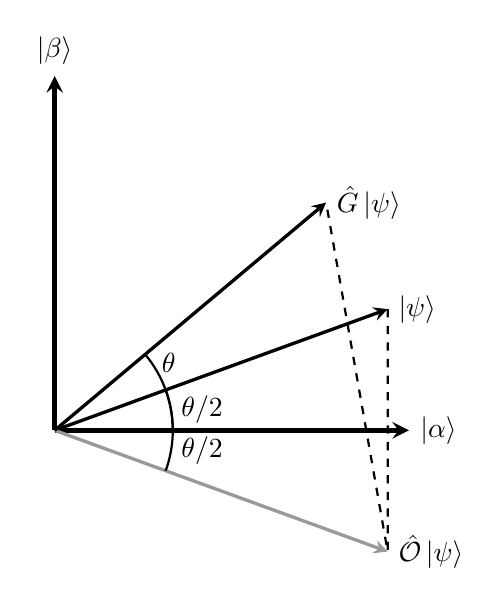
\begin{tikzpicture}
  [scale=1.5,
  axis/.style={ultra thick,->,>=stealth},
  vec/.style={very thick,->,>=stealth},
  angles/.style={thick}]

  % define the angle theta in terms units of degrees
  \def\ang{20}

  % origo
  \coordinate (O) at (0,0);

  % draw axis
  \draw[axis] (O) -- (3,0) node [anchor=west]   {$\ket{\alpha}$};

  \draw[axis] (O) -- (0,3) node [anchor=south]  {$\ket{\beta}$};

  % vectors
  \draw[vec]          (O) -- (\ang:3cm) node [right]
  {$\ket{\psi}$};

  \draw[vec,black!40] (O) -- (-\ang:3cm) node [right,text=black]
  {$\operator\ket{\psi}$};

  \draw[vec]          (O) -- ({2*\ang}:3cm) node [right]
  {$\hat{G}\ket{\psi}$};

  % draw lines connecting the vectors
  \draw[dashed,thick] (\ang:3cm) -- (-\ang:3cm) -- ({2*\ang}:3cm);

  % draw angles
  \draw[angles] (1,0) arc [start angle=0, end angle=\ang, radius=1]
  node[midway, right] {$\theta/2$};

  \draw[angles] (1,0) arc [start angle=0, end angle=-\ang, radius=1]
  node[midway, right] {$\theta/2$};

  \draw[angles] (1,0) arc [start angle=0, end angle={2*\ang}, radius=1]
  node[very near end, right] {$\theta$};
\end{tikzpicture}

	\label{fig:Grover}
	\caption{The action of a single Grover iteration, $G$.}
\end{figure}

%--------------------------------------
%               END
%--------------------------------------
%\bibliographystyle{plain}
%\bibliography{bibliography.bib}
\end{document}
